%-----------------------------------------------------------------------------%
\chapter{\babTiga}
%-----------------------------------------------------------------------------%
%\todo{tambahkan kata-kata pengantar bab 1 disini}


Metodologi penelitian yang akan dilakukan di dalam penelitian ini adalah \textit{Design Science Research Methods and Patterns} \citep{vaishnavi_design_2007}. Metodologi penelitian terdiri dari 5 (lima) tahapan seperti digambarkan pada Gambar \ref{fig:design-science-research-methodology} yaitu: \textit{Awareness of Problem}, \textit{Suggestion}, \textit{Development}, \textit{Evaluation}, dan \textit{Conclusion}.


\begin{figure}[h]
	\centering
	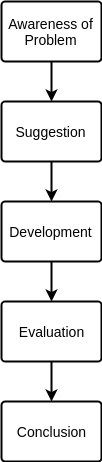
\includegraphics[width=2cm]{Resources/Images/design-science-research-methodology}
	\captionsetup{format=hang}
	\caption{Tahapan \textit{Design Science Research Methods and Patterns}}
	\label{fig:design-science-research-methodology}
\end{figure}


%-----------------------------------------------------------------------------%
\section{\textit{Awareness of Problem}}
%-----------------------------------------------------------------------------%
Langkah pertama dalam \textit{Design Science Research Methods and Patterns} adalah \textit{awareness of problem}. Langkah ini merupakan proses identifikasi dan definisi masalah. Permasalahan yang diidentifikasi dapat tersusun dari permasalahan nyata (\textit{real problem}) maupun permasalahan penelitian (\textit{research problem}). \textit{Real problem} diidentifikasi melalui analisis dan wawancara dengan \textit{subject matter}. Sementara \textit{research problem} diidentifikasi dari riset-riset yang meneliti permasalahan yang terkait dengan \textit{real problem}.


%-----------------------------------------------------------------------------%
\section{\textit{Suggestion}}
%-----------------------------------------------------------------------------%
Setelah masalah terdefinisikan, maka tahapan berikutnya adalah menemukan solusi dari masalah tersebut. Serangkaian analisis dan \textit{preliminary research} dilakukan untuk menemukan kandidat solusi dari permasalahan. Pada tahapan ini, akan diperoleh keluaran berupa \textit{tentative design} atau \textit{design overview}.


%-----------------------------------------------------------------------------%
\section{\textit{Development}}
%-----------------------------------------------------------------------------%
\textit{Tentative design} yang diperoleh pada tahap sebelumnya kemudian dikembangkan dan diimplementasikan pada tahap ini. Elaborasi dari \textit{tentative design} memerlukan kreativitas. Complete design diimplementasikan dalam sejumlah bahasa pemrograman yang bervariasi, kemudian dikombinasikan dengan sejumlah perangkat lunak untuk membentuk sebuah prototipe sistem. Sebuah mekanisme komunikasi juga dipilih pada tahap ini untuk mendukung implementasi dari sistem.


%-----------------------------------------------------------------------------%
\section{\textit{Evaluation}}
%-----------------------------------------------------------------------------%
Prototipe sistem yang diimplementasikan pada tahap sebelumnya kemudian diuji dengan menggunakan serangkaian skenario. Sejumlah data juga digunakan pada tahapan ini. Hasil pengujian kemudian direpresentasikan dalam tabel dan grafik untuk memudahkan dalam menarik kesimpulan.


%-----------------------------------------------------------------------------%
\section{\textit{Conclusion}}
%-----------------------------------------------------------------------------%
Kesimpulan merupakan tahapan akhir dari penelitian. Kesimpulan yang diambil harus dapat menjawab masalah yang telah didefinisikan di awal penelitian.





